% ==========================================
% BAB VI EVALUASI
% ==========================================
\cleardoublepage
\chapter{EVALUASI DAN PEMBAHASAN}
\label{chap:evaluasi}

Bab ini menyajikan hasil dari pengujian sistem Equilibria melalui studi laboratorium terkontrol (\textit{Controlled Lab Study}) dan analisis kesesuaian pelaksanaan proyek. Evaluasi dilakukan untuk mengukur efektivitas sistem dalam meningkatkan hasil belajar siswa serta kemampuannya dalam memitigasi efek \textit{overpersonalization}.

\section{Analisis Kesesuaian Pelaksanaan}
\label{sec:analisis_kesesuaian}

Bagian ini mengevaluasi pelaksanaan proyek dari perspektif manajemen waktu dan anggaran, membandingkan antara rencana awal dengan realisasi aktual selama proses pengembangan sistem.
\subsection{Kesesuaian Linimasa Pelaksanaan}
Realisasi pengembangan sistem secara umum mengalami keterlambatan satu bulan dibandingkan rencana awal. Tahap pengujian (\textit{Controlled Lab Study}) baru dapat dilaksanakan pada minggu pertama Mei 2026. Realisasi jadwal pelaksanaan aktual disajikan pada Gambar \ref{fig:gantt_chart_realisasi} dengan sel berwarna abu-abu menunjukkan alokasi waktu awal dan sel berwarna merah, kuning, dan biru menunjukkan realisasi aktual waktu pengerjaan setiap fase.

\begin{figure}[!ht]
    \centering
    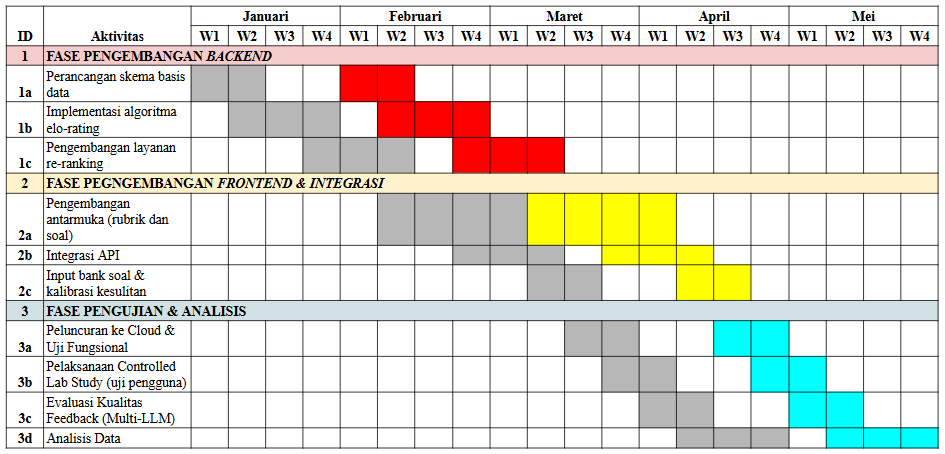
\includegraphics[width=0.85\textwidth]{images/gantt_chart_realization.png}
    % \framebox[0.9\textwidth]{\vbox{\vspace{3cm} \centering [Placeholder: Gantt Chart Realisasi Linimasa Implementasi] \vspace{3cm}}}
    \caption{Gantt Chart Realisasi Pelaksanaan Implementasi dan Pengujian}
    \label{fig:gantt_chart_realisasi}
\end{figure}

\subsection{Kesesuaian Anggaran Biaya}
Realisasi biaya operasional sistem disajikan pada Tabel \ref{tbl:realisasi_rab}. Terjadi efisiensi biaya pada komponen LLM yang tidak digunakan, namun terdapat pengeluaran untuk konsolidasi infrastruktur \textit{cloud} guna menjaga kelancaran pengembangan.

\begin{table}[!ht]
    \centering
    \caption{Realisasi Anggaran Biaya Implementasi}
    \label{tbl:realisasi_rab}
    \begin{tabular}{|p{0.05\textwidth}|p{0.30\textwidth}|p{0.30\textwidth}|p{0.15\textwidth}|}
        \hline
        \textbf{No} & \textbf{Komponen} & \textbf{Spesifikasi/Layanan} & \textbf{Biaya (Rp)} \\
        \hline
        1 & \textit{Consolidated Hosting} & Railway (\textit{Hobby Tier}) & Rp 80.000 \\
        \hline
        2 & \textit{Domain} & Subdomain Provider & Rp 0 \\
        \hline
        3 & Layanan LLM & Tidak digunakan & Rp 0 \\
        \hline
        4 & Perangkat \& Internet & Aset Pribadi / \textit{Sunk Cost} & Rp 0 \\
        \hline
        \multicolumn{3}{|r|}{\textbf{Total Biaya Aktual}} & \textbf{Rp 80.000} \\
        \hline
    \end{tabular}
\end{table}

\section{Prosedur Pengujian Laboratorium (\textit{Lab Study})}
\label{sec:prosedur_pengujian}

Pengujian dilakukan menggunakan metode \textit{Ablation Study Two-Group Pretest Posttest} yang dimodifikasi, dengan pembagian peserta ke dalam Grup A (dengan intervensi kolaboratif) dan Grup B (tanpa intervensi/kontrol). Partisipan terdiri dari 10 mahasiswa yang telah menyelesaikan mata kuliah pemodelan basis data program studi Sistem dan Teknologi Informasi ITB (IF2040), yang kemudian dibagi menjadi dua kelompok. Sesi pengujian berlangsung selama kurang lebih 105 menit yang mencakup tahap \textit{pre-test} untuk kalibrasi awal, interaksi sistem (75 menit), dan tahap akhir untuk pengumpulan umpan balik kualitatif. Berbeda dengan metode klasik, pengujian ini tidak melaksanakan ujian \textit{post-test} secara terpisah, melainkan metrik \textit{post-test} diwakili (diproksi) oleh nilai kemahiran akhir (\textit{final individual theta}) yang dicapai pengguna pada sistem di penghujung sesi interaksi.

\section{Hasil dan Analisis Peningkatan Hasil Belajar}
\label{sec:hasil_belajar}

Efektivitas pembelajaran diukur menggunakan metrik \textit{Normalized Learning Gain} (NLG) untuk membandingkan peningkatan pengetahuan antara Grup A dan Grup B secara objektif.

\subsection{Uji Kesetaraan Awal (\textit{Baseline Equivalence})}
Sebelum mengukur peningkatan hasil belajar, perlu dipastikan bahwa kedua kelompok partisipan memulai pengujian dari titik kemampuan yang setara. Hal ini penting untuk menjamin validitas eksperimen \textit{Two-Group}. Analisis kesetaraan awal dilakukan menggunakan \textit{Mann-Whitney U Test} terhadap nilai praktikum (sebagai representasi kemampuan historis) dan skor \textit{pre-test} (sebagai representasi kemampuan awal pada sistem).

Berdasarkan pengolahan data menggunakan uji statistik non-parametrik \textit{Mann-Whi-\\tney U Test}, diperoleh hasil yang menunjukkan tidak adanya perbedaan yang signifikan antara kedua kelompok sebelum intervensi diberikan. Pada metrik nilai praktikum historis, rata-rata Grup A adalah 47,67 dan Grup B adalah 45,96, dengan nilai $p\text{-value} = 0,7619$ ($p > 0,05$). Serupa dengan hal tersebut, pada skor \textit{pre-test} di dalam sistem, rata-rata kemahiran awal Grup A berada pada angka 1313,33 dan Grup B pada angka 1300,00, dengan nilai $p\text{-value} = 0,9062$ ($p > 0,05$). Hasil ini membuktikan bahwa Grup A dan Grup B memulai pengujian dari titik kemahiran yang setara secara statistik, sehingga asumsi ekuivalensi dasar pada metode \textit{Two-Group} terpenuhi. Hal ini menjamin bahwa perbedaan peningkatan performa (\textit{gain}) di akhir sesi dapat diatribusikan secara valid pada efek keberadaan intervensi kolaboratif.

\subsection{Perbandingan Skor Pre-test dan Post-test}
Mengingat asesmen dilakukan secara terintegrasi, skor \textit{pre-test} dan proksi \textit{post-test} direpresentasikan menggunakan skala \textit{Elo rating} ($\theta$). Untuk menghitung metrik NLG menggunakan skala ini, digunakan dua pendekatan batas maksimum: 

\begin{enumerate}
    \item \textbf{Teoretis:} Menggunakan nilai \textit{Elo} maksimal sebesar 1500 (berdasarkan rentang kesulitan sistem pada studi \textcite{Vesin2022}).
    \item \textbf{Empiris:} Menggunakan nilai \textit{Elo} tertinggi yang secara empiris dicapai oleh peserta selama pengujian sebagai batas maksimum.
\end{enumerate}

Tabel \ref{tbl:perbandingan_skor} menyajikan rekapitulasi skor rata-rata berdasarkan skala \textit{Elo} tersebut, beserta nilai NLG teoretis dan empirisnya.

\begin{table}[!ht]
    \centering
    \caption{Perbandingan Skor Rata-rata Pre-test dan Post-test}
    \label{tbl:perbandingan_skor}
    \begin{tabular}{|p{2.5cm}|p{2cm}|p{2cm}|p{2cm}|p{2cm}|}
        \hline
        \textbf{Kelompok} & \textbf{Rata-rata Pre-test} & \textbf{Rata-rata Post-test} & \textbf{NLG Teoretis} & \textbf{NLG Empiris} \\
        \hline
        \hline
        Grup A (Intervensi) & 1313,33 & 1445,08 & 0,69 & 0,57 \\
        \hline
        Grup B (Kontrol) & 1300,00 & 1236,59 & -0,21 & -0,19 \\
        \hline
    \end{tabular}
\end{table}

\subsection{Analisis Signifikansi Peningkatan (NLG)}
Berdasarkan Tabel \ref{tbl:perbandingan_skor}, terlihat bahwa Grup A mengalami peningkatan hasil belajar yang sangat positif, dengan nilai NLG Teoretis sebesar $0,69$ dan NLG Empiris sebesar $0,57$. Merujuk pada kriteria interpretasi Hake, nilai ini tergolong ke dalam kategori peningkatan sedang hingga tinggi (\textit{medium to high gain}). Sebaliknya, Grup B justru mengalami penurunan performa dengan nilai NLG Teoretis $-0,21$ dan Empiris $-0,19$. Penurunan skor pada grup kontrol ini secara empiris mengindikasikan terjadinya kelelahan kognitif (\textit{cognitive fatigue}) atau demotivasi akibat terjebak berulang kali dalam soal-soal sulit (\textit{stagnasi}) tanpa adanya bantuan eksternal.

Untuk menguji signifikansi perbedaan metrik tersebut, dilakukan analisis statistik menggunakan \textit{Mann-Whitney U Test}. Hasil pengujian menunjukkan bahwa nilai $p\text{-value}$ untuk distribusi skor NLG adalah $0,0095$. Karena nilai $p < 0,05$, maka Hipotesis Nol ($H_0$) ditolak. Dapat disimpulkan secara meyakinkan bahwa keberadaan intervensi kolaboratif memberikan dampak yang positif dan signifikan secara statistik terhadap peningkatan hasil belajar siswa dibandingkan dengan kelompok yang hanya belajar mandiri.

\section{Hasil dan Analisis Efektivitas Mitigasi \textit{Overpersonalization}}
\label{sec:hasil_mitigasi}

Analisis ini berfokus pada kemampuan sistem dalam mendeteksi stagnasi dan mengembalikan momentum pertumbuhan kemahiran siswa melalui intervensi kolaboratif.

\subsection{Analisis Perubahan Kemahiran (\textit{Slope} \texorpdfstring{$\Delta\theta$}{Delta Theta})}
Evaluasi dilakukan dengan membandingkan gradien (\textit{slope}) perubahan skor Elo sebelum dan sesudah intervensi pada titik stagnasi terdeteksi.

\begin{figure}[!ht]
    \centering
    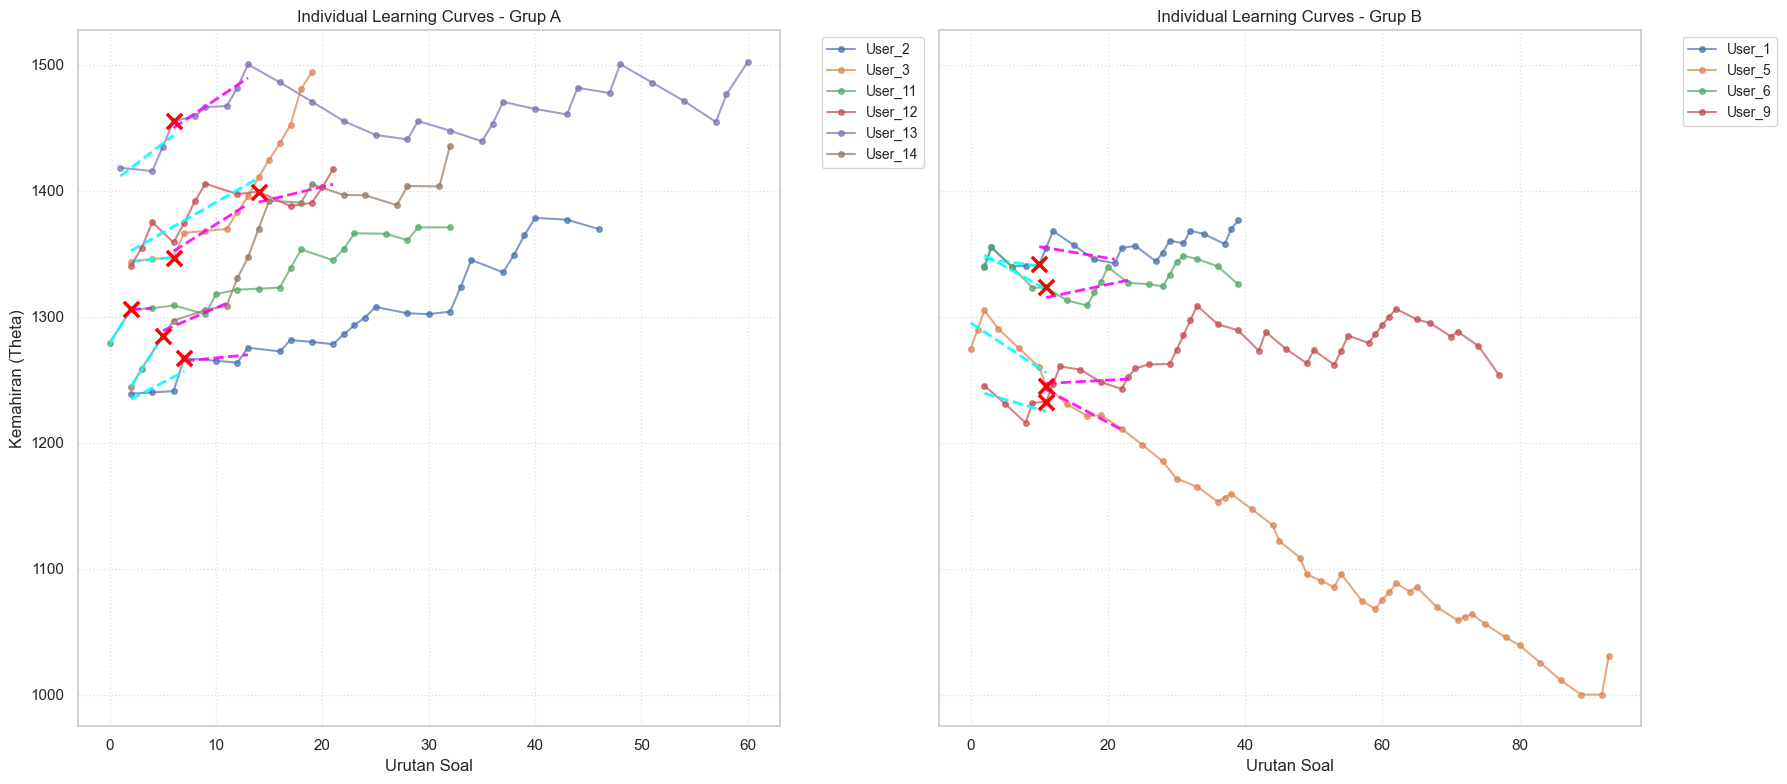
\includegraphics[width=1\textwidth]{images/individual_trajectories_with_trendline.png}
    \caption{Visualisasi Perubahan Momentum Belajar Sebelum dan Sesudah Titik Pertama Stagnasi}
    \label{fig:slope_comparison}
\end{figure}

Berdasarkan visualisasi pada Gambar \ref{fig:slope_comparison}, terlihat adanya perubahan tren pergerakan kemahiran (\textit{trajectory}) antara fase sebelum (\textit{pre}) dan sesudah (\textit{post}) titik stagnasi. Temuan ini dikonfirmasi oleh fakta statistik bahwa rerata gradien tren kemahiran (\textit{slope post-intervention}) pengguna Grup A secara konsisten kembali naik dengan rata-rata perbedaan gradien positif sebesar $+0,67$ setelah titik stagnasi. Di sisi lain, meskipun secara matematis Grup B mencatatkan rata-rata perbedaan gradien akhir yang juga positif ($+1,01$), nilai tersebut bersifat semu karena memiliki simpangan baku yang sangat besar ($SD = 2,47$). Pemeriksaan data individual menunjukkan bahwa angka ini terdistorsi oleh satu partisipan pencilan (\textit{outlier}) yang mengalami lonjakan ekstrem, sedangkan mayoritas partisipan Grup B lainnya mencatatkan pertumbuhan yang nyaris datar (mendekati nol). Distribusi peningkatan Grup A yang jauh lebih merata ($SD = 0,68$), menunjukkan indikasi positif terkait efektivitas intervensi dalam mengembalikan momentum belajar yang konsisten dan lebih merata bagi seluruh populasi kelompok yang sebelumnya mengalami stagnasi.

\subsection{Validitas Pemicuan Stagnasi (\textit{Trigger Rate})}
Mekanisme deteksi stagnasi yang menggunakan ambang batas variansi $\epsilon = 165$ pada awalnya dirancang untuk mendeteksi pola \textit{learning plateau}. Berdasarkan data log pengujian, tingkat keberhasilan pemicuan mencapai 100\%, artinya seluruh pengguna di Grup A berhasil memicu mekanisme kolaboratif ini (dengan rata-rata 15 kejadian stagnasi per pengguna). Hal ini secara nominal melampaui target awal pelaksanaan pengujian yang mengharapkan setidaknya 50\% pengguna mendapatkan kesempatan intervensi. Namun, tingginya angka pemicuan ini mengekspos sebuah kelemahan desain sistem yaitu, parameter variansi yang ditetapkan ternyata terlalu sensitif (\textit{hypersensitive}). Sebagai gambaran ekstrem, rata-rata 30 kejadian stagnasi (seperti yang dicatat oleh data internal sistem untuk pengguna Grup B) dalam rentang pengujian yang hanya berisi sekitar 60 aktivitas pengerjaan soal mengimplikasikan bahwa sistem mendeteksi stagnasi belajar hampir di setiap dua soal. Secara pedagogis, frekuensi interupsi seketat ini kurang masuk akal karena fluktuasi kognitif minor atau jeda berpikir normal pengguna rentan tertafsirkan sebagai stagnasi akut.

Meskipun algoritma utamanya terbukti terlalu sensitif, kombinasi dengan pemicu cadangan (\textit{fallback trigger} pada $N=9$ aktivitas terakhir) tetap memberikan jaring pengaman (\textit{safety net}) komprehensif. Secara konseptual, keberadaan \textit{fallback trigger} memastikan bahwa pengguna dengan profil skor yang sangat fluktuatif ke arah bawah akibat perilaku menebak asal, yang secara matematis luput dari deteksi \textit{variance} konvergen, tetap terjamin mendapatkan intervensi. Berdasarkan analisis \textit{syslogs} sistem, pemicu cadangan ini sebenarnya tidak pernah aktif selama sesi pengujian karena seluruh kejadian stagnasi telah tercakup oleh algoritma variansi yang hipersensitif. Namun demikian, keberadaan mekanisme gabungan ini secara aktual terbukti berhasil memecah isolasi pembelajaran tanpa ada satu pun siswa Grup A yang luput dari pantauan sistem.

\section{Hasil dan Analisis Komponen Kolaboratif}
\label{sec:hasil_kolaborasi}

Bagian ini mengevaluasi kualitas interaksi sosial yang terjadi dalam sistem serta validitas algoritma \textit{Social Elo} dan mekanisme \textit{Re-ranking}.

\subsection{Validitas Algoritma \textit{Constraint-based Re-ranking}}
Algoritma \textit{Re-ranking} dirancang untuk secara spesifik memastikan bahwa pengguna yang sedang mengalami stagnasi tidak dipasangkan dengan sejawat yang memiliki tingkat kompetensi identik, guna memastikan terjadinya transfer pengetahuan yang bermakna. Berdasarkan ekstraksi data \textit{syslogs} sistem terkait kejadian (\textit{events}) pembuatan sesi kolaboratif, tercatat 10 kali pemicuan pencarian sejawat heterogen (\textit{find\_heterogeneous\_peer}) yang berhasil. 

Data log menunjukkan bahwa perbedaan kemahiran absolut (\textit{theta difference}) antara peminta (\textit{requester}) dan peninjau (\textit{reviewer}) memiliki rata-rata sebesar $112,56$ poin Elo. Lebih penting lagi, validasi terhadap indeks \textit{Effect Size} menunjukkan bahwa seluruh pasangan menghasilkan nilai \textit{Cohen's d} di atas batas minimal desain ($d \geq 0,5$), dengan nilai terendah $d = 0,61$ dan rata-rata keseluruhan mencapai $d = 1,186$ (kategori efek sangat besar). Metrik ini mengonfirmasi bahwa algoritma sistem telah berfungsi dengan tepat dan sesuai dengan kerangka teoretis, yakni berhasil mencegah isolasi kompetensi dengan menyajikan keberagaman sudut pandang dari sejawat yang memiliki perbedaan pemahaman yang signifikan secara statistik.

\subsection{Kualitas Umpan Balik Sejawat (\textit{Peer Feedback Quality})}
Kualitas umpan balik dievaluasi berdasarkan skor yang dihasilkan oleh mesin NLP (\textit{system\_score}) dan penilaian subjektif penerima (\textit{is\_helpful}).

\begin{table}[!ht]
    \centering
    \caption{Statistik Kualitas Umpan Balik Kolaboratif}
    \label{tbl:social_quality}
    \begin{tabular}{|l|c|}
        \hline
        \textbf{Metrik} & \textbf{Nilai Rata-rata} \\
        \hline
        Skor Sistem (NLP) & 0,404 \\
        \hline
        Tingkat Kebergunaan (\textit{Helpfulness Rate}) & 100\% \\
        \hline
    \end{tabular}
\end{table}

\subsection{Konvergensi \textit{Social Elo}}
Perhitungan skor Elo Sosial pada sistem terbukti mampu menguantifikasi kualitas umpan balik sejawat. Dengan mengandalkan perhitungan NLP yang divalidasi oleh penerima ulasan, nilai $\theta_{social}$ untuk setiap pengguna berubah secara dinamis. Rata-rata persentase \textit{thumbs up} yang menyentuh angka absolut 100\% mengindikasikan bahwa responden sangat menghargai bantuan dari sejawatnya. Meskipun demikian, dijumpai suatu fenomena keterbatasan dalam durasi pengujian singkat ini (75 menit), yaitu skala $\theta_{social}$ pada beberapa pengguna belum mencapai konvergensi yang matang sehingga pemanfaatannya dalam porsi bobot $\theta_{display}$ (sebesar 20\%) belum sepenuhnya terlihat memisahkan rentang pemeringkatan antar siswa dengan jelas. Pada implementasi skala riilnya nanti, fitur ini akan memerlukan partisipasi jangka panjang agar model pemeringkat kolaboratifnya lebih matang dan stabil.

\section{Pembahasan Umum dan Implikasi}
\label{sec:pembahasan_umum}

Analisis dari hasil pengujian menegaskan satu hal penting: membiarkan siswa belajar secara terisolasi dengan sistem asesmen adaptif konvensional menyimpan risiko \textit{overpersonalization} berupa isolasi akademik (\textit{filter bubble}). Ketika siswa berulang kali dihadapkan pada materi yang dinilai "sesuai" namun sesungguhnya memicu stagnasi karena mereka tidak kunjung mampu memecahkan masalah, sistem yang pasif hanya akan mencatat penurunan skor tanpa memberikan jalan keluar. Sebagaimana yang ditunjukkan oleh tren penurunan gradien elo-rating pada Grup B, isolasi ini menyebabkan frustrasi dan mematikan momentum pertumbuhan belajar siswa. Fenomena empiris ini sejalan dengan kerangka teoretis yang diajukan oleh \textcite{Bahg2025}, yang memperingatkan bahwa algoritma personalisasi sering kali mengorbankan diversitas informasi dan membatasi eksposur pengguna terhadap perspektif alternatif. Dalam konteks pembelajaran, lingkungan yang terlampau dipersonalisasi (\textit{hyper-personalized}) dapat mendistorsi pemahaman siswa terhadap ruang masalah, mendorong pengambilan sampel informasi yang bias, serta memicu generalisasi pengetahuan yang keliru (\textit{inaccurate generalization}) yang sering kali justru diiringi oleh rasa percaya diri yang semu (\textit{overconfidence}).

Sebaliknya, keberadaan mekanisme intervensi terautomasi (\textit{automated intervention}) pada Grup A berhasil memutus siklus stagnasi tersebut. Dengan "memaksa" terjadinya pertukaran perspektif melalui konten \textit{peer-review} secara terkalibrasi, sistem tidak hanya berhasil mendiversifikasi eksposur siswa, tetapi secara statistik terbukti membangkitkan kembali grafik pertumbuhan kemahiran mereka. Terlihat dari perubahan gradien yang positif setelah titik terdeteksinya stagnasi dan nilai positif NLG yang signifikan secara statistik.

Implikasi dari studi ini menunjukkan bahwa desain sistem \textit{e-learning} ke depannya tidak cukup lagi hanya dengan merekomendasikan soal yang selaras dengan kemahiran, melainkan harus memiliki fitur mitigasi sosial proaktif. Umpan balik kualitatif tambahan dari mahasiswa menunjukkan bahwa interupsi proaktif dari sistem membantu meringankan beban psikologis bagi siswa yang merasa "malu/takut" untuk bertanya langsung pada sejawat. Adanya batasan anonimitas yang diatur secara algoritmik (\textit{Constraint-based Re-ranking}) memberikan dorongan positif bagi mereka untuk meninjau kueri secara objektif tanpa bias. Hal ini meletakkan fondasi baru bagi perancangan sistem pendidikan adaptif yang lebih kolaboratif dan manusiawi.


